\documentclass[11pt]{article}
\usepackage{natbib,mybigpackage}
\usepackage{algorithm}
%\usepackage{program}
%\usepackage{algpseudocode}
\usepackage{algorithmic}
\usepackage{listings}

\usepackage{amsmath}


\def\xbf{\mathbf{x}}
\def\zbf{\mathbf{z}}
\def\xibf{\mathbf{\xi}}
\title{MA 226 - Assignment Report 7}
\author{Ayush Sharma\\150123046}
\begin{document}
\titlepage
\newpage
\begin{enumerate}
\item[Q 1.] Generate 50 randam numbers from Geometric distribution of the form :
$$f(x;p) = pq^{i-1} \hspace{10mm} i = 1,2,... \hspace{10mm} 0 < p < 1.$$
Draw the probability mass function.
\end{enumerate}

\noindent{Solution:}
In Geometric distribution with parameter p, we have $P(X=i) = pq^{i-1} , i \leq 1$.\\
Note that the cumulative probability $P(X \leq j) = \sum_{i=1}^{j} P(X=i) = 1 - q^{j}$.\\
Generate $U \sim \mathcal{U}(0,1)$ and set $X = j$ if $1 - q^{j-1} \leq U < 1 - q^{j}$.\\
$U \sim \mathcal{U}(0,1) \Rightarrow (1 - U) \sim \mathcal{U}(0,1)$.\\
\begin{equation}
\begin{split}
X	& = min\{j | q^{j} < 1 - U\}\\
	& = min\{j | j \times log(q) < log(1 - U)\}\\
	& = min\{j | j > \frac{log(1 - U)}{log(q)}\}\\
	& = min\{j | j > \frac{log(1 - U)}{log(q)}\}\\
	& = \left \lceil {\frac{log(1 - U)}{log(q)}} \right \rceil
\end{split}
\end{equation}

\noindent{Code for R}
\begin{lstlisting}
genGeometric <- function(sample, p) {
	u <- runif(sample,0,1);
	G <- ceiling(log(u)/log(1-p));
	return (G);
}

set.seed(1);
p = runif(1,0,1);	#Taking value of 'p', i.e. probability for success in a trial .

sample = 50;

G <- genGeometric(sample, p);	#Generating Geometric Random Numbers.
Density <- p * ((1 - p)^(G - 1));

cat("The value of p taken is",p,".\n");
cat("The sample mean and variance, for the", sample, "random numbers generated from Geometric distribution, with parameter p =", p, ", are calculated to be", mean(G),",and",var(G),"respectively.\n");

pdf("1.pdf");
#plot(G, Density, xlab = "x", ylab = "p(x)", main = paste("Probability mass function\nGeometric distribution, n =", sample), col = "red");
plot(G, Density, xlab = "x", ylab = "p(x)", main = "", col = "red");
legend("topright", legend = paste("parameter", p), lty = 0, col = "red", bty = 'n');
\end{lstlisting}

\noindent{\textbf{Results}:}\\
The plots can be shown as :
\begin{figure}[H]
	\centering
	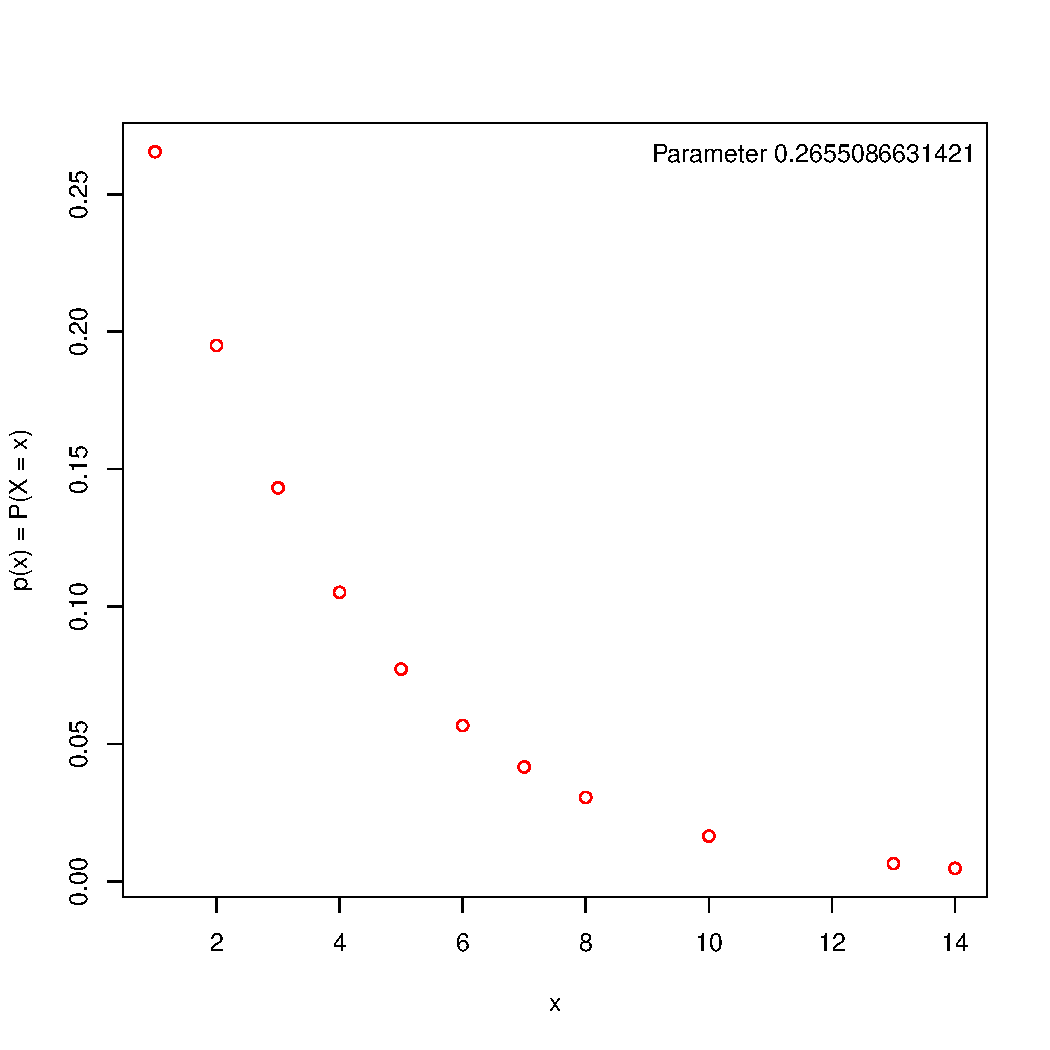
\includegraphics[width=0.7\textwidth]{1.pdf}
		\caption{Probability mass function for 50 samples from Geometric distribution}
\end{figure}

The value of p taken is 0.2655087.\\
The sample mean and variance, for the 50 random numbers generated from Geometric distribution, with parameter p = 0.2655087, are calculated to be 3.42 ,and 8.615918 respectively.\\
These values are close to the theoretical ones, $\frac{1}{p} = \frac{1}{0.2655087} = 3.766355$, and $\frac{1 - p}{p^2} = \frac{1 - 0.2655087}{0.2655087^2} = 10.41907$.
\newpage
\begin{enumerate}
\item[Q 2.] Generate 50 random numbers from Poisson distribution with mean 2. Draw the probability mass function and the cumulative distribution function.
\end{enumerate}

\noindent{Solution:} 
In the case of Poisson, we exploit the recursion property $p_{i+1} = \frac{\lambda}{i + 1}p_i$, for $i \geq 0$.
\begin{algorithm}[H]
\caption{Generating Random number from Poisson distribution with parameter $\lambda$.}
\begin{algorithmic}[1]
\STATE Generate $U$ from $\mathcal{U}(0,1)$.
\STATE Set $i = 0$, $p = e^{-l}$ and $F = p$.
\IF {$U < F$}
	\STATE $X = i$.
\ELSE
	\STATE Set $p = \frac{\lambda}{i + 1}p$, $F = F + p$ and $i = i + 1$.
	\STATE Return to step 3.
\ENDIF
\end{algorithmic}
\end{algorithm}

\noindent{Code for R}
\begin{lstlisting}
genPoisson <- function(sample, l) {
	P <- vector(length = sample);
	for (j in 1:sample) {
		u = runif(1,0,1);
		i = 0;
		p = exp(-l);
		F = p; 
		repeat {
			if (u < F) {
				P[j] = i;
				break;
			}
			else {
				p = ((l * p) / (i + 1));
				F = F + p;
				i = i + 1;
			}
		}
	}
	return (P);	
}

set.seed(1);

sample = 50;
l = 2;

P <- genPoisson(sample, l);
s_P <- sort(P);

Density <- ((exp(-l) * (l^(P))) / factorial(P));

cat("The sample mean and variance, for the", sample, "Poisson random numbers generated, are calculated to be", mean(P), ",and", var(P), "respectively.\n");

pdf("2_pmf.pdf");
#plot(P, Density, xlab = "x", ylab = "p(x) = P(X = x)", main = paste("Probability mass function\nPoisson distribution (with mean 2), n =", sample), col = "red");
plot(P, Density, xlab = "x", ylab = "p(x) = P(X = x)", main = "", col = "red");

pdf("2_CDF.pdf");
#plot(ecdf(s_P), xlab = "x", ylab = "F(x) = P(X <= x)", do.points = FALSE, main = paste("Cumulative distribution function\nPoisson distribution (with mean 2), n =", sample), col = "red");
plot(ecdf(s_P), xlab = "x", ylab = "F(x) = P(X <= x)", do.points = FALSE, main = "", col = "red");
\end{lstlisting}
\newpage
\noindent{\textbf{Results}:}\\
The plots can be shown as :
\begin{figure}[H]
	\centering
	\subfloat[Probability mass function for 50 samples]{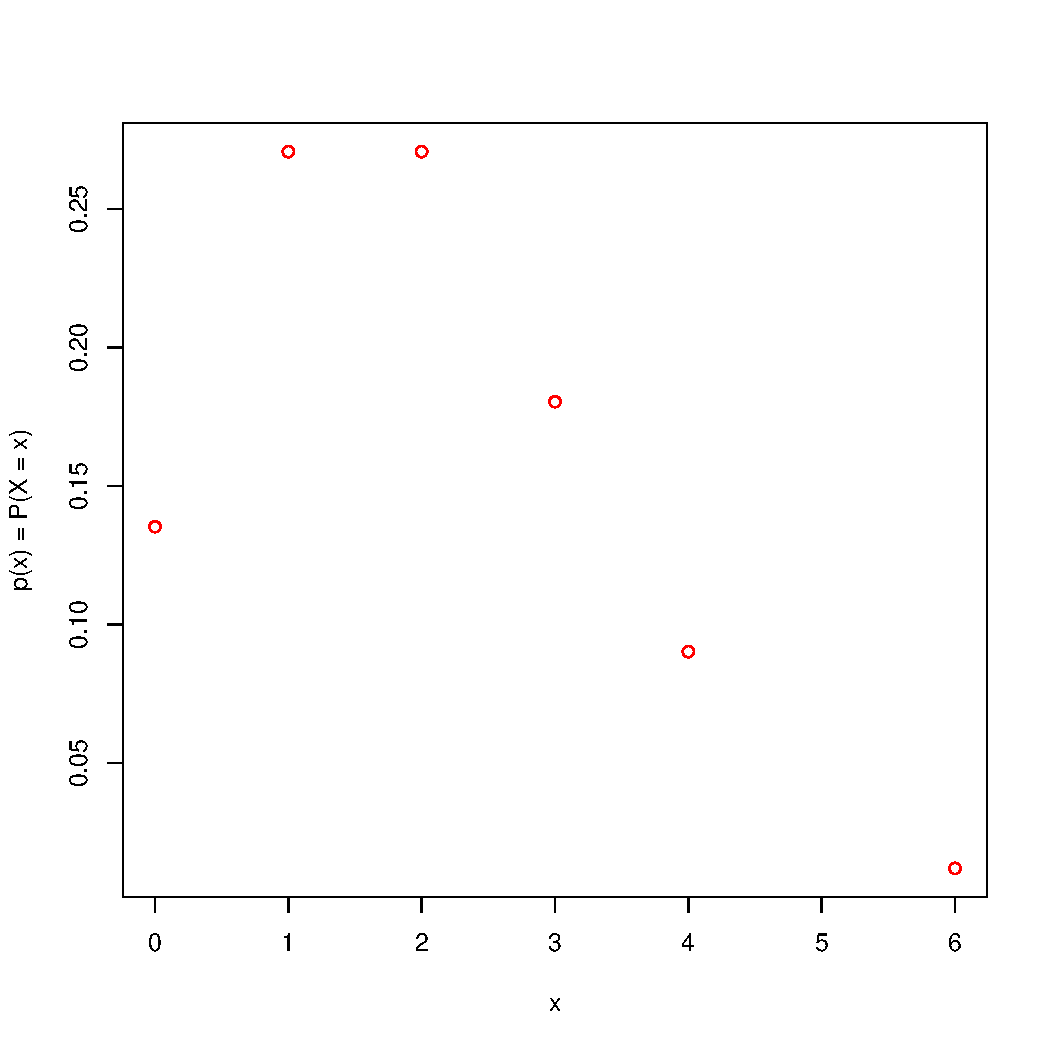
\includegraphics[width=0.55\textwidth]{2_pmf.pdf}}
	\subfloat[Cumulative Distribution Function for 50 samples]{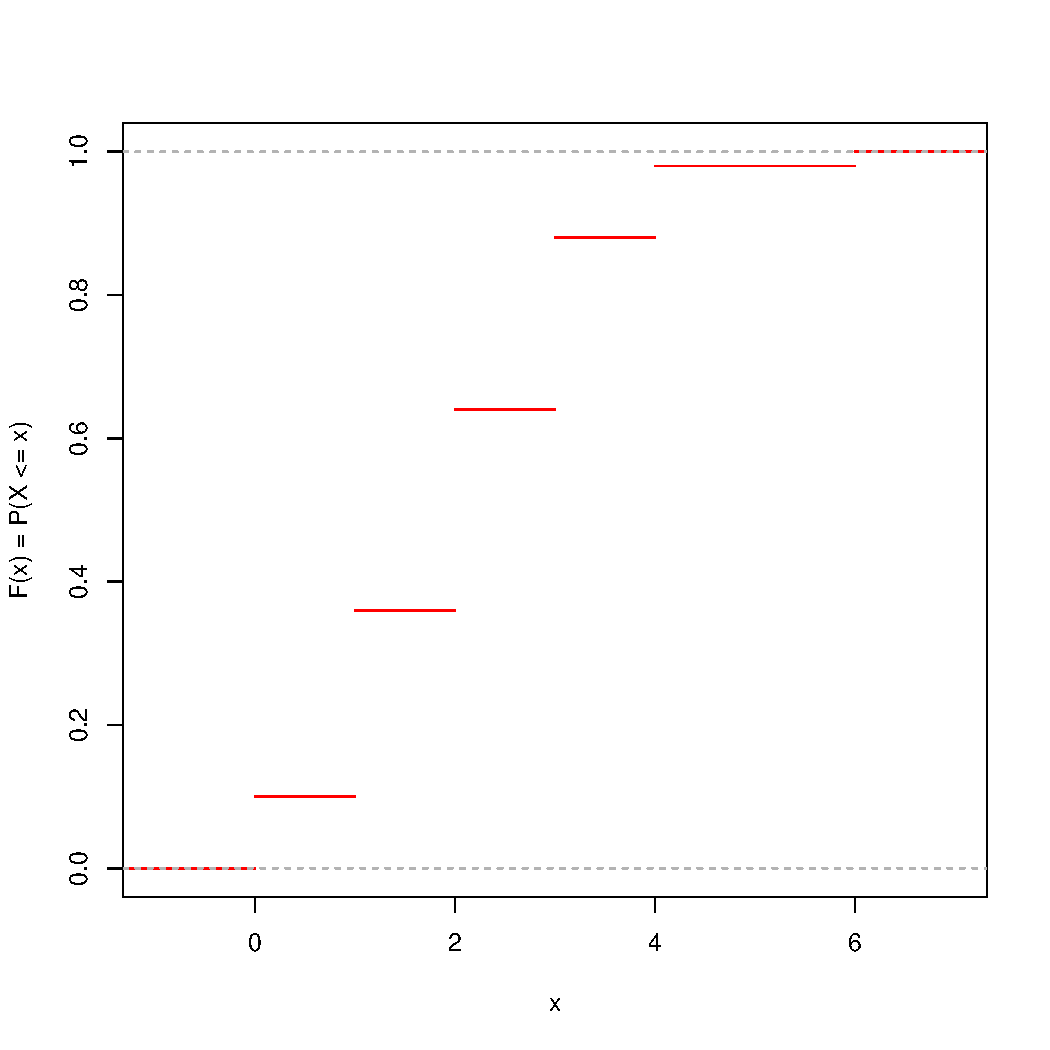
\includegraphics[width=0.55\textwidth]{2_CDF.pdf}}
		\caption{Poisson distribution with $\lambda = 2$}
\end{figure}

The sample mean and variance, for the 50 Poisson random numbers generated, are calculated to be 2.06 ,and 1.649388 respectively.
These values are close to the theoretical ones, $\lambda = 2$.
\newpage
\begin{enumerate}
\item[Q 3.] Draw the histogram based 50 generated random numbers from the mixture of two Weibull distributions :
$$f(x;\beta_{1},\theta_{1},\beta_{2},\theta_{2},p) = pf_{1}(x;\beta_{1},\theta_{1}) + (1 - p)f_{2}(x;\beta_{2},\theta_{2})$$
where $f_{1}(.)$ and $f_{2}(.)$ are two Weibull distributions of the form : $f(x;\beta,\theta) = \beta\theta^{\beta}x^{\beta-1}e^{-(\theta x)^{\beta}}$ where, $\beta_{1} = 2, \theta_{1} = 1, \beta_{2} = 1.5, \theta_{2} = 1, p = 0.4$.
\end{enumerate}

\noindent{Solution:}
Consider simulating from a distribution with mass function $P(X=j) = \alpha p_{j}^{(1)} + (1 - \alpha) p_{j}^{(2)}$, $j \leq 0$, $0 < \alpha < 1$.\\
If $X_1$ and $X_2$ are the random variables with respective mass functions $p_{j}^{(1)}$ and $p_{j}^{(2)}$, then
$$X = \begin{cases} X_1 & \text{with probability $\alpha$} \\ X_2 & \text{with probability $(1 - \alpha)$} \end{cases}$$
Generating random number from Weibull distributions of the form $f(x;\beta,\theta) = \beta\theta^{\beta}x^{\beta-1}e^{-(\theta x)^{\beta}}$ :\\
Then $F(x;\beta,\theta) = 1 - e^{-(\theta x)^{\beta}}$.
And, using Inverse Transform Method, $X = \frac{1}{\theta}(-log(1-U))^{\frac{1}{\beta}}$ where, $U \sim \mathcal{U}(0,1)$.

\begin{algorithm}[H]
\caption{Generating random number from the mixture of given two Weibull distributions.}
\begin{algorithmic}[1]
\STATE Generate $U_1, U_2$ from $\mathcal{U}(0,1)$.
\IF {$U_1 < p$}
	\STATE Generate $X_1$ from the relation $X_1 = \frac{1}{\theta_1}(-log(1-U_2))^{\frac{1}{\beta_1}}$.
	\STATE $X = X_1$.
\ELSE
	\STATE Generate $X_2$ from the relation $X_2 = \frac{1}{\theta_2}(-log(1-U_2))^{\frac{1}{\beta_2}}$.
	\STATE $X = X_2$.
\ENDIF
\end{algorithmic}
\end{algorithm}
\newpage
\noindent{Code for R}
\begin{lstlisting}
genWeibull <- function(val, beta, theta) {
	return ((1/theta) * ((-log(1 - val))^(1/beta)));
}

genMix <- function(sample, beta_1, theta_1, beta_2, theta_2, p) {
	M <- vector(length = sample);
	for (i in 1:sample) {
		u <- runif(2,0,1);
		if (u[1] < p) {
			M[i] = genWeibull(u[2], beta_1, theta_1);
		}
		else {
			M[i] = genWeibull(u[2], beta_2, theta_2);
		}
	}
	return (M);
}

set.seed(1);

sample = 50;

M <- genMix(sample, 2, 1, 1.5, 1, 0.4);

cat("The sample mean and variance, for the", sample, "random numbers generated from mixture of the two given Weibull distributions, are calculated to be", mean(M), ",and", var(M),"respectively.\n");

pdf("3.pdf");
#hist(M, xlab = "x", breaks = 50, main = paste("Histogram of Mixed Distribution\nn =", sample), col = "red");
hist(M, xlab = "x", main = "", col = "red");
\end{lstlisting}
\newpage
\noindent{\textbf{Results}:}\\
The histogram can be shown as :
\begin{figure}[H]
	\centering
	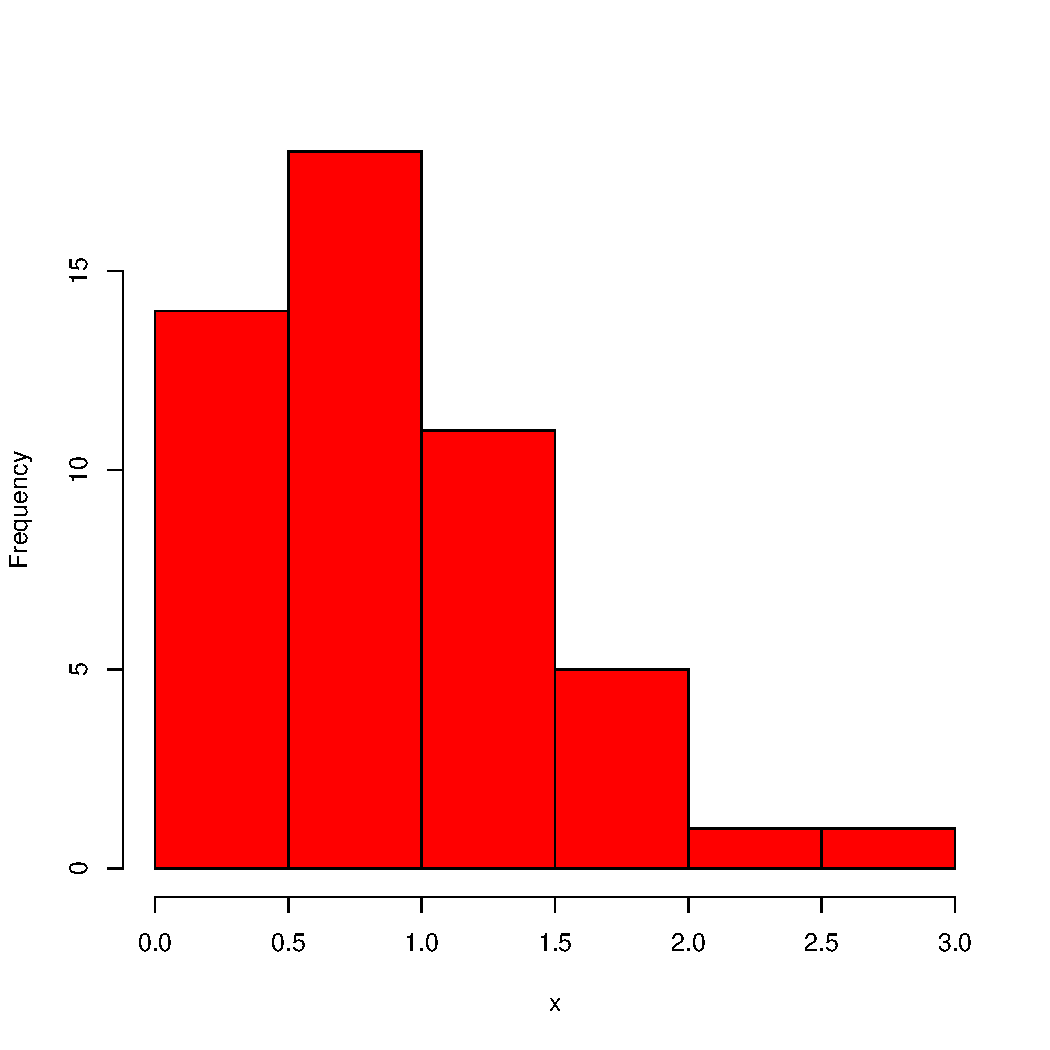
\includegraphics[width=0.7\textwidth]{3.pdf}
		\caption{Histogram of Mixed Distribution for 50 samples}
\end{figure}

The sample mean and variance, for the 50 random numbers generated from mixture of the two given Weibull distributions, are calculated to be 0.8864908 ,and 0.305633 respectively.
\end{document}

%#Made by Ayush Sharma#
%#Signed as AShar#